% The three cases of Thomassen's proof (generated by figs_c1ch07.py).
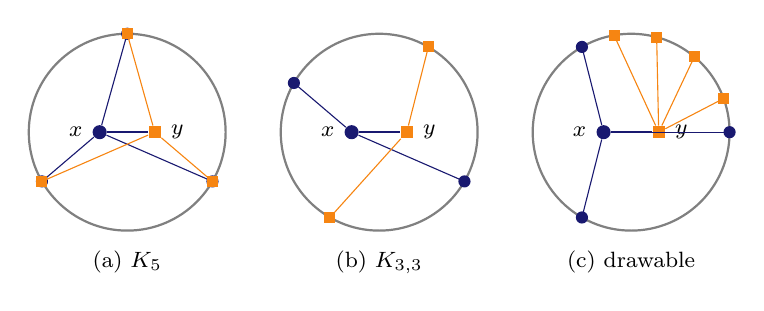
\begin{tikzpicture}[x=1cm,y=1cm,v/.style={circle,fill=MidnightBlue,inner sep=1.8pt},w/.style={rectangle,fill=BurntOrange,inner sep=2.2pt},e/.style={thick,MidnightBlue},l/.style={font=\footnotesize}]
\draw[thick,gray] (0,0) circle (1.25);
\node[circle,fill=MidnightBlue,inner sep=1.8pt,label={[l]left:$x$}] (xa) at (-0.35,0) {};
\node[rectangle,fill=BurntOrange,inner sep=2.2pt,label={[l]right:$y$}] (ya) at (0.35,0) {};
\draw[e] (xa) -- (ya);
\draw[MidnightBlue] (xa) -- (0.000,1.250); \fill[MidnightBlue] (0.000,1.250) circle (2.2pt);
\draw[MidnightBlue] (xa) -- (-1.083,-0.625); \fill[MidnightBlue] (-1.083,-0.625) circle (2.2pt);
\draw[MidnightBlue] (xa) -- (1.083,-0.625); \fill[MidnightBlue] (1.083,-0.625) circle (2.2pt);
\draw[BurntOrange] (ya) -- (0.000,1.250); \fill[BurntOrange] (-0.070,1.180) rectangle (0.070,1.320);
\draw[BurntOrange] (ya) -- (-1.083,-0.625); \fill[BurntOrange] (-1.153,-0.695) rectangle (-1.013,-0.555);
\draw[BurntOrange] (ya) -- (1.083,-0.625); \fill[BurntOrange] (1.013,-0.695) rectangle (1.153,-0.555);
\node[l] at (0,-1.65) {(a) $K_5$};
\draw[thick,gray] (3.2,0) circle (1.25);
\node[circle,fill=MidnightBlue,inner sep=1.8pt,label={[l]left:$x$}] (xb) at (2.85,0) {};
\node[rectangle,fill=BurntOrange,inner sep=2.2pt,label={[l]right:$y$}] (yb) at (3.5500000000000003,0) {};
\draw[e] (xb) -- (yb);
\draw[MidnightBlue] (xb) -- (2.117,0.625); \fill[MidnightBlue] (2.117,0.625) circle (2.2pt);
\draw[MidnightBlue] (xb) -- (4.283,-0.625); \fill[MidnightBlue] (4.283,-0.625) circle (2.2pt);
\draw[BurntOrange] (yb) -- (3.825,1.083); \fill[BurntOrange] (3.755,1.013) rectangle (3.895,1.153);
\draw[BurntOrange] (yb) -- (2.575,-1.083); \fill[BurntOrange] (2.505,-1.153) rectangle (2.645,-1.013);
\node[l] at (3.2,-1.65) {(b) $K_{3,3}$};
\draw[thick,gray] (6.4,0) circle (1.25);
\node[circle,fill=MidnightBlue,inner sep=1.8pt,label={[l]left:$x$}] (xc) at (6.050000000000001,0) {};
\node[rectangle,fill=BurntOrange,inner sep=2.2pt,label={[l]right:$y$}] (yc) at (6.75,0) {};
\draw[e] (xc) -- (yc);
\draw[MidnightBlue] (xc) -- (5.775,1.083); \fill[MidnightBlue] (5.775,1.083) circle (2.2pt);
\draw[MidnightBlue] (xc) -- (5.775,-1.083); \fill[MidnightBlue] (5.775,-1.083) circle (2.2pt);
\draw[MidnightBlue] (xc) -- (7.650,0.000); \fill[MidnightBlue] (7.650,0.000) circle (2.2pt);
\draw[BurntOrange] (yc) -- (7.575,0.428); \fill[BurntOrange] (7.505,0.358) rectangle (7.645,0.498);
\draw[BurntOrange] (yc) -- (7.203,0.958); \fill[BurntOrange] (7.133,0.888) rectangle (7.273,1.028);
\draw[BurntOrange] (yc) -- (6.724,1.207); \fill[BurntOrange] (6.654,1.137) rectangle (6.794,1.277);
\draw[BurntOrange] (yc) -- (6.183,1.231); \fill[BurntOrange] (6.113,1.161) rectangle (6.253,1.301);
\node[l] at (6.4,-1.65) {(c) drawable};
\end{tikzpicture}
